\documentclass[12pt]{article}


% Math		****************************************************************************************
\usepackage{fancyhdr} 
\usepackage{amsfonts}
\usepackage{amsmath}
\usepackage{amsthm}
\usepackage{dsfont}

% Macros	****************************************************************************************
\usepackage{calc}

% Commands	****************************************************************************************
\newcommand{\problem}[1]{\hspace{-4 ex} \large \textbf{#1}\\}

%page		****************************************************************************************
\usepackage[margin=1in]{geometry}
\usepackage{setspace}
\doublespacing
\pagestyle{fancy}
\fancyhf{}
\rhead{Shaw \space \thepage}
\setlength\parindent{0pt}


%Images		****************************************************************************************
\usepackage{graphicx}
\graphicspath{ {images/} }


\begin{document}
	\thispagestyle{empty}
	
	\begin{flushright}
		Sage Shaw \\
		m527 - Fall 2017 \\
		\today
	\end{flushright}
	
{\large \textbf{HW 3: Section 5.4: \#4, 16, 17, 20; and Section 5.5: \#4 }}\bigbreak
\large{\textbf{Section 5.4}}\\
\problem{\#4} Find a general solution in terms of $J_v$ and $J_{-v}$.
\begin{align}\label{eq1}
y^{\prime\prime} + (e^{-2x}-\frac{1}{9})y = 0
\end{align}
	We would like to manipulate this so that it matches Bessel's equation
	$$
	x^2y^{\prime\prime} + xy^\prime +(x^2-v^2)y = 0
	$$
	To do so we will substitute like so: $z=e^{-x}$. Then we can derive the following:
	\begin{align*}
		\frac{dz}{dx} & = -e^{-x} = -z &  \frac{dy}{dx} & = \frac{dy}{dz}\frac{dz}{dx}= -e^{-x}\frac{dy}{dz}\\
		\frac{d^2z}{dx^2} & = e^{-x} = z & \frac{d^2y}{dx^2} & = \frac{d^2z}{dx^2}\frac{dy}{dz} + \Big(\frac{dz}{dx}\Big)^2\frac{d^2y}{dz^2}= z\frac{dy}{dz} + z^2\frac{d^2y}{dz^2}
	\end{align*}
	Substituting into (\ref{eq1}) we have
	$$
	\Big(z\frac{dy}{dz} + z^2\frac{d^2y}{dz^2}\Big) + \Big(z^2 - \Big(\frac{1}{3}\Big)^2\Big)y = 0
	$$
	Rearranging, we obtain an equation in the form of Bessel's equation:
	\begin{align}\label{eq2}
		z^2\frac{d^2y}{dz^2} + z\frac{dy}{dz} + \Big(z^2 - \Big(\frac{1}{3}\Big)^2\Big)y & = 0
	\end{align}
	We know that $J_{\frac{1}{3}}(z)$ and $J_{-\frac{1}{3}}(z)$ are solutions to (\ref{eq2}) since $\frac{1}{3} \notin \mathbb{Z}$. Substituting $z=e^{-x}$ we obtain our general solution
	$$
	y(x) = C_1J_{\frac{1}{3}}(e^{-x}) + C_2J_{-\frac{1}{3}}(e^{-x})
	$$
	In Table 1 are shown several example solutions to our differential equation.
	\begin{table}
		\centering
		\begin{tabular}{cc}
			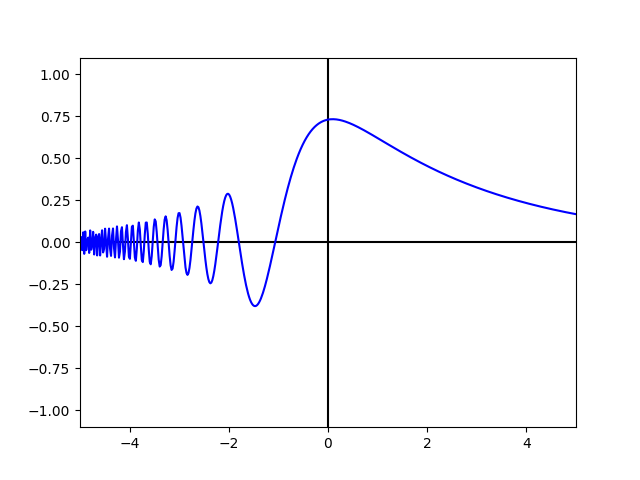
\includegraphics[width=.5\textwidth]{hw3_figure_1} & 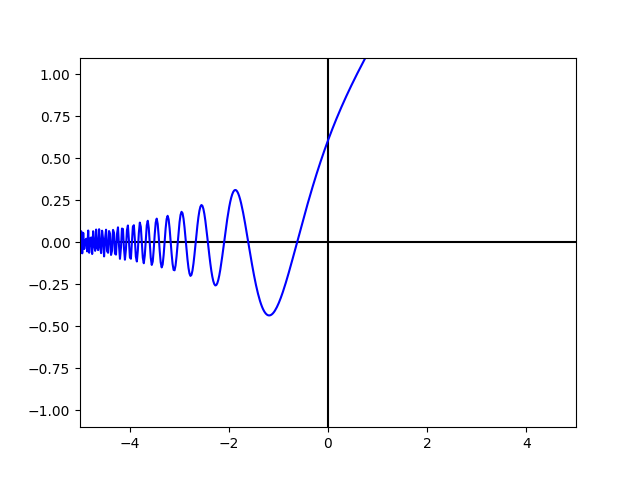
\includegraphics[width=.5\textwidth]{hw3_figure_2} \\
			$C_1=1$ and $C_2=0$ & $C_1=0$ and $C_2=1$ \\
			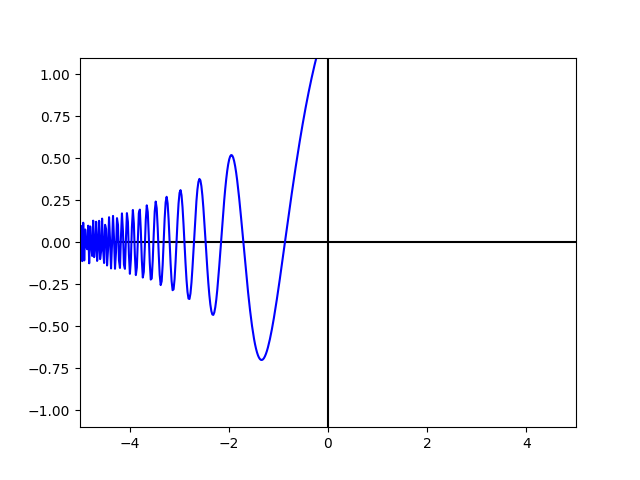
\includegraphics[width=.5\textwidth]{hw3_figure_3} & 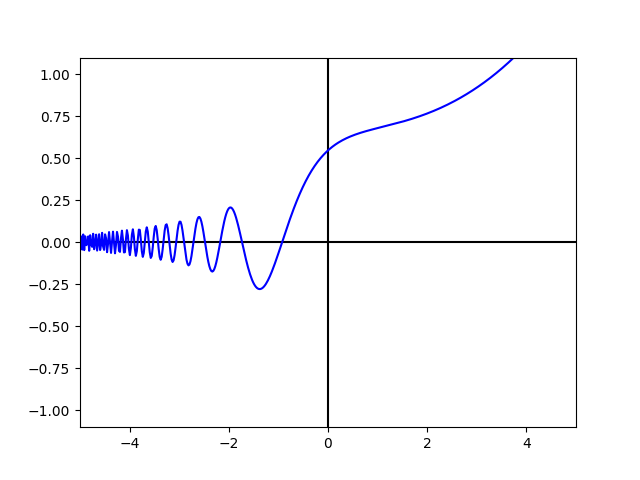
\includegraphics[width=.5\textwidth]{hw3_figure_4} \\
			$C_1=1$ and $C_2=1$ & $C_1=.5$ and $C_2=.3$ \\
		\end{tabular}
		\caption{Example solutions to equation (\ref{eq1})}
		\label{tbl:table_of_figures}
	\end{table} 
	
\problem{\#16} 

\end{document}
